%
% path-finding user interfaces
% @author Tobias Weber <tweber@ill.fr>
% @date july-2021
% @license see 'LICENSE' file
%

\chapter{User Interfaces}
\label{ch:gui}

The software of the present work has been realised in a modular fashion, it comprises a core
module (see chapter \ref{ch:impl}), which can be easily used as a library and linked into 
external C++ applications. More details on the core library can be found in section \ref{sec:library}.
Such a library usage will be important in the future when we plan to utilise the software as a 
plug-in module to the instrument control software \textit{NOMAD} \cite{web_NOMAD} that is 
employed at the Institut Laue-Langevin.

Furthermore, a graphical user interface (GUI) has been implemented for a visual and interactive 
representation of the instrument and the underlying algorithms. 
The GUI is described in detail in section \ref{sec:gui}.

Finally, the software allows scripting via \textit{Python} \cite{Rossum2011, web_python}. 
Apart from simply setting up a workflow and plotting the results, the \textit{Python} interface 
will allow the usage of the software in \textit{Python}-based instrument control systems such as 
\textit{NICOS} \cite{web_NICOS}, which is used at the Forschungsreaktor M\"unchen II (FRM-II). 
Details on the scripting interface can be found in section \ref{sec:scripting}.



\section{Core module and C++ library}
\label{sec:library}
The core module comprises all necessary calculation as well as input and output sub-modules. 
Here, we only describe the latter two, since the computation functionality of the core module 
has already been treated in chapter \ref{ch:impl}.

The instrument configuration is read from an \textit{XML} file whose hierarchical structure
mirrors the internal data organisation of the core module and its class hierarchy.
The \textit{XML} file is parsed using the \textit{Boost.PropertyTree} library \cite{web_boost_proptree}
and objects are created of the respective classes once the corresponding section in the \textit{XML}
structure is discovered. An \textit{XML} section is handed down to the corresponding \textit{C++} object,
so that each object only receives the portions of the \textit{XML} configuration it is responsible for.
Editing the \textit{XML} instrument configurations can be done using the GUI module of section \ref{sec:gui}.

While the central \lstinline[language=C++]|PathBuilder| class offers getter functions for all intermediate
data that is generated during each step of the calculation workflow, the final results are output using
the classes derived from the purely virtual class \lstinline[language=C++]|PathsExporterBase| that resides
in the files \lstinline|./src/core/PathsExporter[.h,.cpp]|. Currently, three possible output classes
are available:
\begin{itemize}
	\item \lstinline[language=C++]|PathsExporterRaw|, which outputs the vertices of the calculated 
		final instrument path in a raw text format.
	\item \lstinline[language=C++]|PathsExporterNomad|, which writes out commands for driving the
		motors of instruments which are controlled by the \textit{NOMAD} software \cite{web_NOMAD}.
	\item \lstinline[language=C++]|PathsExporterNicos|, which generates \textit{Python} code to
		be used for driving the instrument using the \textit{NICOS} \cite{web_NICOS} control system.
\end{itemize}
For easy extensibility and to isolate the \lstinline[language=C++]|PathBuilder| class from the output
code, the output class hierarchy is realised using the Visitor pattern \cite{wiki_visitor}, where
the \lstinline[language=C++]|PathBuilder| accepts the output base class and dispatches to the
desired child object.

The core module functionality is self-contained and does, for instance, not depend on any GUI code.
It is therefore straightforward to statically or dynamically link it to external applications which 
wish to use the path-finding functionality. To avoid exposing the user to the complexities of 
the \textit{C++} language, a more comfortable approach is provided by both the graphical as well 
as the \textit{Python} interface, which are described in the following sections.



\section{Graphical user interface}
\label{sec:gui}

The software's main graphical user interface (GUI), for which a typical session is depicted
in Fig. \ref{fig:gui}, is based on the \textit{Qt} framework \cite{web_Qt}, which allows
for an easy and rapid cross-platform GUI development in \textit{C++}. We support both
current releases of \textit{Qt}, namely version 5 and version 6.
Similar to the core calculation module, the GUI is written in the recent \textit{C++20}
standard \cite{ISOCPP20} of the C++ language family \cite{Stroustrup2008, Stroustrup2018}.
The source code of the GUI module can be found in the directory \lstinline|./src/gui| of the
source repository, see chapter \ref{ch:online} for more information.

\begin{figure}[htb]
		\begin{center}
			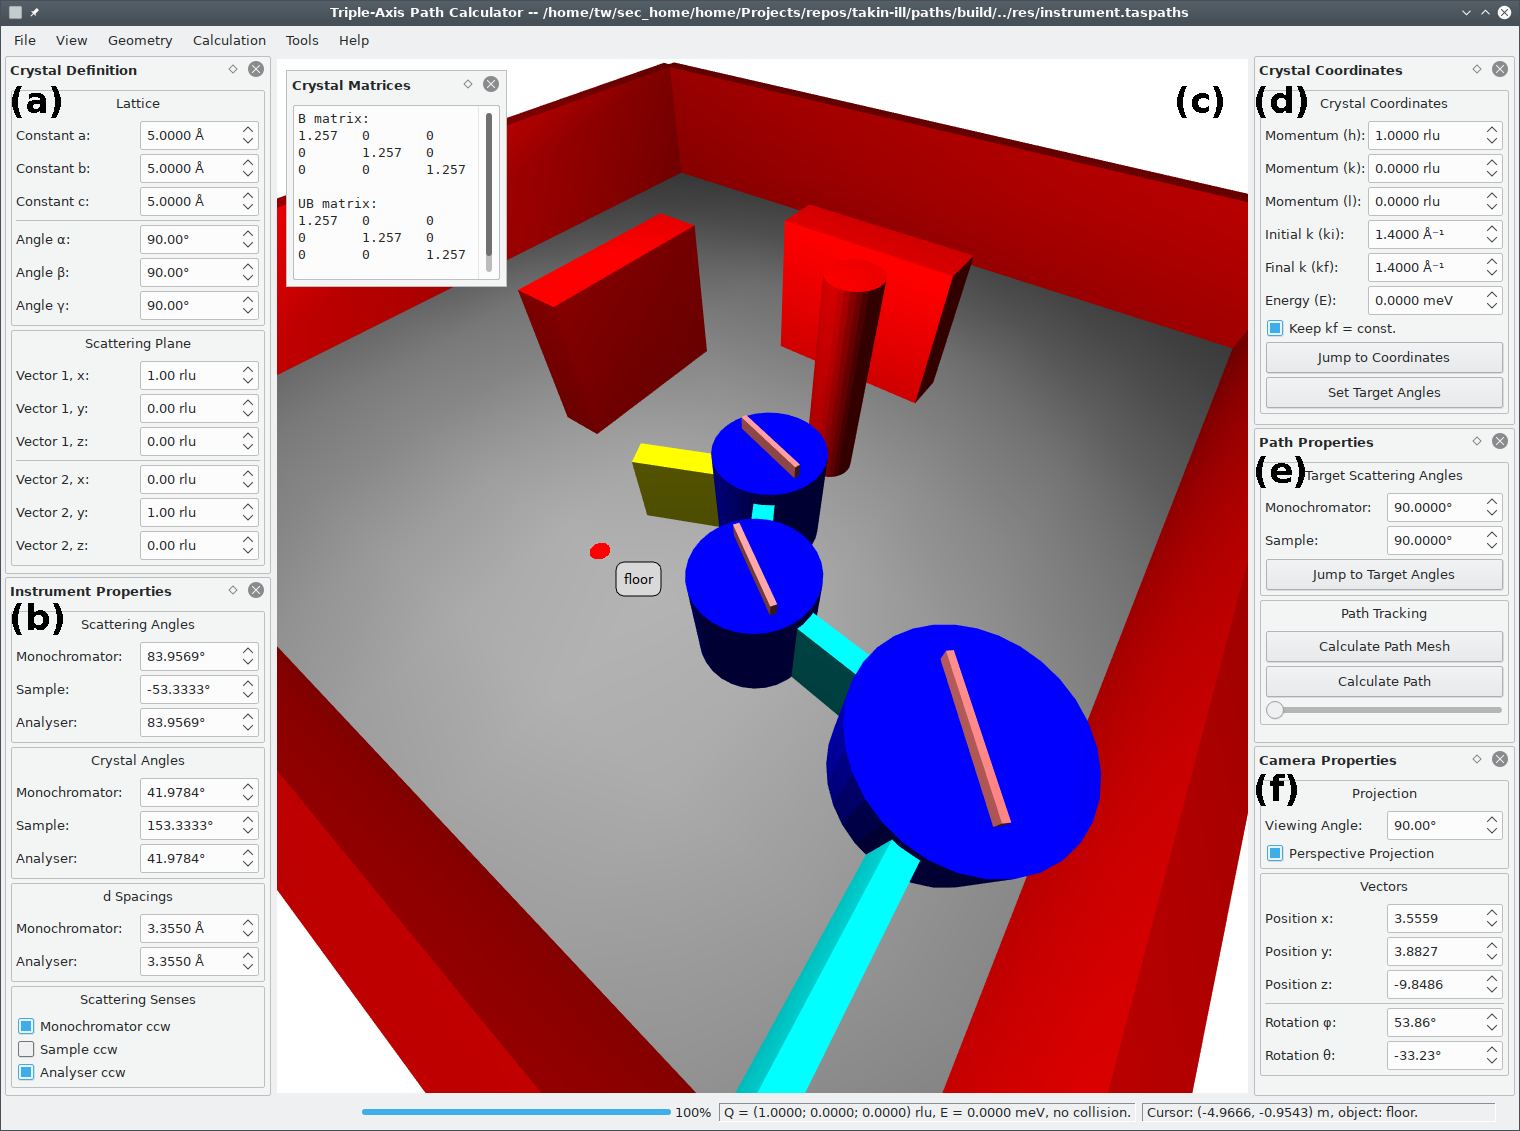
\includegraphics[width = 1 \textwidth]{figures/gui}
		\end{center}
	\caption[Main program GUI.]{Main GUI. Here, instrument and sample crystal properties can be set up,
		walls can be added and moved and paths around them be calculated.
		The central view provides a three-dimensional visualisation of the instrument
		configuration and is fully dynamic: Every element, including the instrument
		and the wall segments, can be moved or manipulated using the mouse.
		\label{fig:gui}}
\end{figure}

The GUI allows the set-up of an instrument configuration and a crystal $UB$ matrix from a
sample definition according to the formalism described in chapter \ref{ch:xtal}.
All calculation is performed in the core module, which is described in chapter \ref{ch:impl}
and to which the GUI is just that, an interface. By the same token, the core module itself is
completely independent of the GUI, or any other interface code, and the full functionality
of the software, except GUI-specific visualisations, is equally accessible from the other
alternative interface modules, e.g. the \textit{Python} interface described in section
\ref{sec:scripting}, or the raw \textit{C++} library interface. Graphical display of the
instrument and the walls as well as the interaction with these elements is performed
using \textit{OpenGL} \cite{web_OpenGL} via Qt's \lstinline[language=C++]|QOpenGLWidget|
\cite{web_QOpenGLWidget} class.



\begin{figure}[htb]
		\begin{center}
			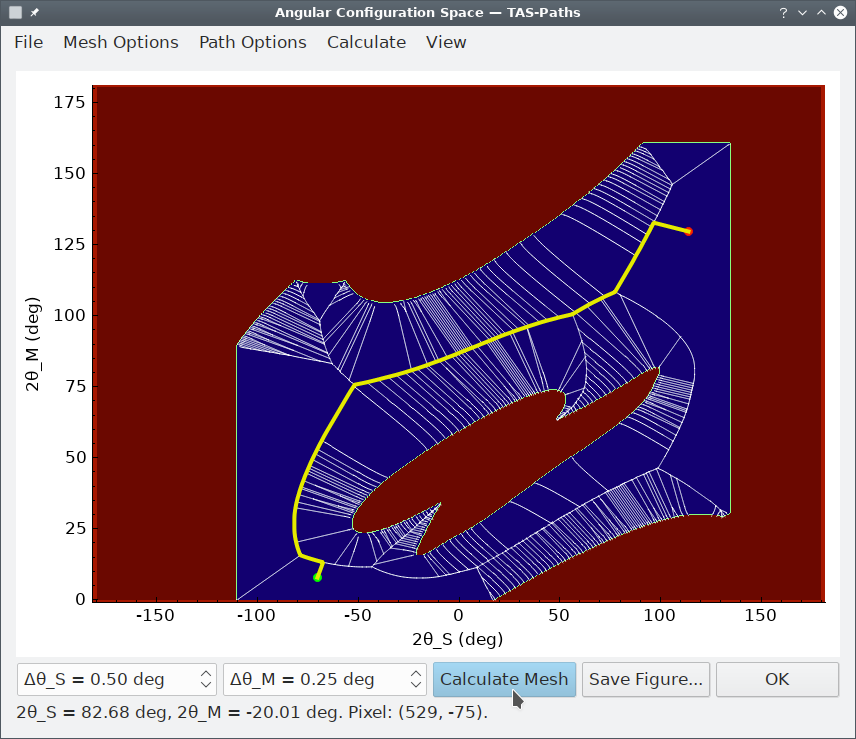
\includegraphics[width = 0.66 \textwidth]{figures/gui_configspace}
		\end{center}
	\caption[Configuration space dialog.]{Angular configuration space and path calculation. The figure plots all
	possible instrument positions for the monochromator and sample scattering angles,
	$2\theta_M$ and $2\theta_S$, respectively. Forbidden positions are shown in red.
	These can be invalid angles as well as collisions of the instrument with walls
	(here, specifically, the pillar from Fig \ref{fig:gui}), or with itself.
	Allowed positions are drawn in blue. The mesh of all possible instrument
	paths is shown as white lines, while a currently selected example path from
	the red start to the green target position is shown as a yellow line.
		\label{fig:gui_configspace}}
\end{figure}





\section{Python scripting interface}
\label{sec:scripting}

In order to allow for a simple inclusion of the core module (see section \ref{sec:library}) of the present 
software in other tools, a scripting interface has been developed using the interface generator \textit{SWIG} \cite{web_swig}. 
\textit{SWIG} is a tool which parses \textit{C} or \textit{C++} header files and creates a native interface 
for several possible scripting languages, of which we opted for \textit{Python} \cite{Rossum2011, web_python} 
as it has become the most popular programming language in neutron science over the last decade.
As the core module already has the structure of a library, the effort to offer scripting functionality
was minimal. Only a few helper functions had to be included in several classes, because \textit{SWIG}
is not yet fully \textit{C++20} compliant and had some problems with new language features such as 
template concepts \cite{TODO}.
The \textit{SWIG} interface definition, which maps the \textit{C++} classes to corresponding Python classes of the same name, 
can be found in the file \lstinline|./scripting/taspaths.i| of the source repository.

An example of the full workflow of loading an instrument definition file, creating a path mesh and finding
the path from a start position in crystal coordinates to a target position is given in listings \ref{lst:pyworkflow1}, \ref{lst:pyworkflow2} and \ref{lst:pyworkflow3}.
The native core module is imported into \textit{Python} as the name \lstinline[language=C++]|tas| on line 9 of the script,
instances of its classes are generated for the individual functionalities.
Specifically, the instrument space class from chapter \ref{sec:tasmodel}, which is the representation of the instrument 
and which is furthermore responsible for the local instrument axis coordinate systems, collision detection, as well as 
loading and saving of instrument configurations, is created on line 37. 
Next, the triple-axis and single-crystal calculator class from chapter \ref{ch:xtal} is created on line 51 and is 
used to set-up the instrument scattering senses and a single-crystal coordinate system.
Finally, the path builder class, which has been described in chapter \ref{sec:buildpath}, is created on line 64 
and used in the rest of the script to calculate the path mesh as
well as the concrete path between the given crystal coordinate points.
The results of the script are shown in Fig. \ref{fig:pyworkflow}, where we employ \textit{Matplotlib} \cite{web_matplotlib} 
to plot the calculated path and the obstacles in configuration space.

\begin{figure}[htb]
		\begin{center}
			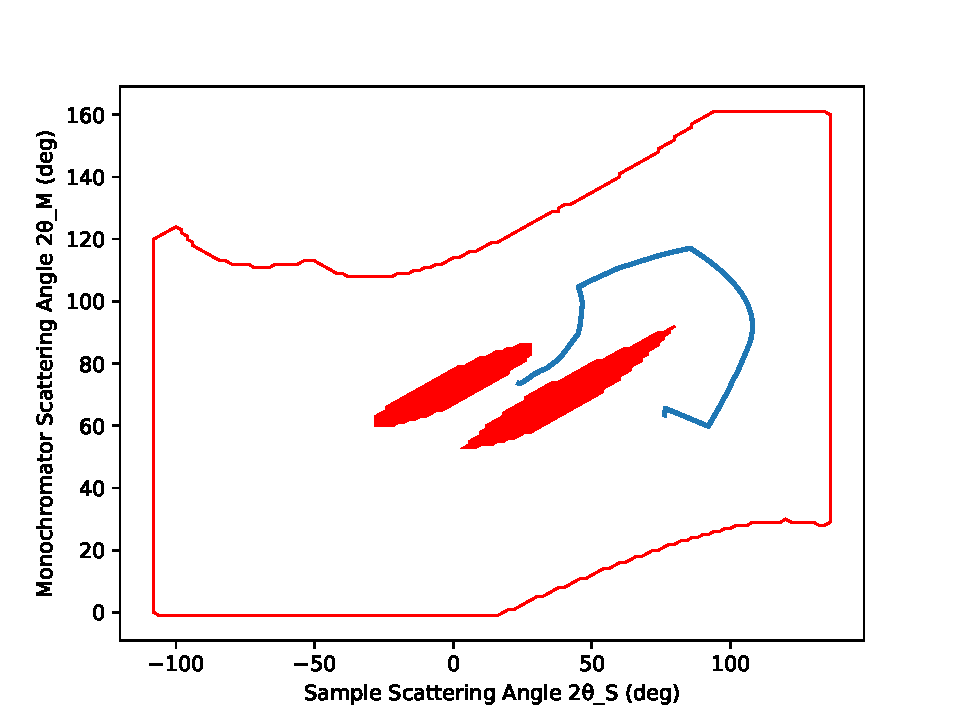
\includegraphics[width = 0.66 \textwidth]{figures/pyworkflow}
		\end{center}
	\caption[Python workflow results.]{Results from the \textit{Python} workflow example of listings
		\ref{lst:pyworkflow1}, \ref{lst:pyworkflow2} and \ref{lst:pyworkflow3}, directly plotted 
		in \textit{Python} using \textit{Matplotlib} \cite{web_matplotlib}.
		The obstacles are shown as red regions, the calculated instrument path is shown as a blue curve.
		\label{fig:pyworkflow}}
\end{figure}


\begin{listing}[htb]
	\begin{lstlisting} [language = Python, 
		basicstyle = {\scriptsize},
		breaklines = true, tabsize = 4,
		numbers = left, firstnumber = 1, numberstyle={\scriptsize}]
import sys
import os
import math as m

cwd = os.getcwd()
sys.path.append(cwd)

# import native C++ core module
import taspaths as tas

# -----------------------------------------------------------------------------
# helper functions
# -----------------------------------------------------------------------------
def error(msg):
	print("Error: %s" % msg)
	exit(-1)

def warning(msg):
	print("Warning: %s" % msg)
# -----------------------------------------------------------------------------

# -----------------------------------------------------------------------------
# options
# -----------------------------------------------------------------------------
write_pathmesh = False
write_path = False
show_plot = True
file_name = "../res/instrument.taspaths"
# -----------------------------------------------------------------------------

# -----------------------------------------------------------------------------
# load instrument
# -----------------------------------------------------------------------------
print("Loading instrument definition...")

# create the instrument space and load an instrument definition
instrspace = tas.InstrumentSpace()
[file_ok, file_date] = tas.InstrumentSpace.load(file_name, instrspace)

if file_ok:
	print("Loaded \"%s\", dated %s." % (file_name, file_date))
else:
	error("Could not load \"%s\"." % (file_name))

print("Instrument definition loaded.\n")
# -----------------------------------------------------------------------------

# -----------------------------------------------------------------------------
# set-up a sample single-crystal
# -----------------------------------------------------------------------------
tascalc = tas.TasCalculator()
tascalc.SetScatteringSenses(True, False, True)
tascalc.SetSampleLatticeConstants(5, 5, 5)
tascalc.SetSampleLatticeAngles(90, 90, 90, True)
tascalc.UpdateB()
tascalc.UpdateUB()
# -----------------------------------------------------------------------------
	\end{lstlisting}
	\caption[Python workflow example 1/3.]{Script showing an example workflow in \textit{Python}.
	Part 1 of 3: Set-up of the instrument and the sample crystal.
	\label{lst:pyworkflow1}}
\end{listing}



\begin{listing}[htb]
	\begin{lstlisting} [language = Python, 
		basicstyle = {\scriptsize},
		breaklines = true, tabsize = 4,
		numbers = left, firstnumber = 58, numberstyle={\scriptsize}]
# -----------------------------------------------------------------------------
# build path mesh
# -----------------------------------------------------------------------------
print("Building path mesh...")

# create the paths builder object
builder = tas.PathsBuilder()
builder.AddConsoleProgressHandler()
builder.SetInstrumentSpace(instrspace)
builder.SetTasCalculator(tascalc)
print("Path builder uses %d threads." % builder.GetMaxNumThreads())

# angular ranges to probe
angle_padding = 4.
a2_delta = 1./180.*m.pi
a4_delta = 2./180.*m.pi
a2_begin = 0. - angle_padding*a2_delta
a2_end = m.pi + angle_padding*a2_delta
a4_begin = -m.pi - angle_padding*a4_delta
a4_end = m.pi + angle_padding*a4_delta

if not builder.CalculateConfigSpace(
	a2_delta, a4_delta,
	a2_begin, a2_end,
	a4_begin, a4_end):
	error("Angular configuration space could not be calculated.")

if not builder.CalculateWallContours(True, False):
	error("Obstacle contours could not be calculated.")

if not builder.CalculateLineSegments():
	error("Line segments could not be calculated.")

if not builder.CalculateVoronoi(False):
	error("Voronoi diagram could not be calculated.")

print("Finished building path mesh.\n")
# -----------------------------------------------------------------------------

# -----------------------------------------------------------------------------
# set-up the start and target coordinates of a path
# -----------------------------------------------------------------------------
print("Calculating path...")

tascalc.SetKf(1.4)
start_angles = tascalc.GetAngles(0.5, 0., 0., 1.)
target_angles = tascalc.GetAngles(1.5, -0.5, 0., 2.5)

# take absolute angles
start_angles.monoXtalAngle = abs(start_angles.monoXtalAngle)
start_angles.sampleXtalAngle = abs(start_angles.sampleXtalAngle)
start_angles.sampleScatteringAngle = abs(start_angles.sampleScatteringAngle)
target_angles.monoXtalAngle = abs(target_angles.monoXtalAngle)
target_angles.sampleXtalAngle = abs(target_angles.sampleXtalAngle)
target_angles.sampleScatteringAngle = abs(target_angles.sampleScatteringAngle)

print("Start angles: a1 = %.2f deg, a5 = %.2f deg, a3 = %.2f deg, a4 = %.2f deg." % (
	start_angles.monoXtalAngle / m.pi*180.,
	start_angles.anaXtalAngle / m.pi*180.,
	start_angles.sampleXtalAngle / m.pi*180.,
	start_angles.sampleScatteringAngle / m.pi*180.))

print("Target angles: a1 = %.2f deg, a5 = %.2f deg, a3 = %.2f deg, a4 = %.2f deg." % (
	target_angles.monoXtalAngle / m.pi*180.,
	target_angles.anaXtalAngle / m.pi*180.,
	target_angles.sampleXtalAngle / m.pi*180.,
	target_angles.sampleScatteringAngle / m.pi*180.))
# -----------------------------------------------------------------------------
	\end{lstlisting}
	\caption[Python workflow example 2/3.]{Script showing an example workflow in \textit{Python}.
	Part 2 of 3: Calculation of the path mesh and the start and target positions from their crystal coordinates.
	\label{lst:pyworkflow2}}
\end{listing}


\begin{listing}[htb]
	\begin{lstlisting} [language = Python, 
		basicstyle = {\scriptsize},
		breaklines = true, tabsize = 4,
		numbers = left, firstnumber = 126, numberstyle={\scriptsize}]
# -----------------------------------------------------------------------------
# find path
# -----------------------------------------------------------------------------
path = builder.FindPath(
		start_angles.monoXtalAngle * 2., start_angles.sampleScatteringAngle,
		target_angles.monoXtalAngle * 2., target_angles.sampleScatteringAngle)
if not path.ok:
	error("No path could be found.")

builder.SetSubdivisionLength(0.5)
vertices = builder.GetPathVerticesAsPairs(path, True, True)

print("Finished calculating path.\n")
# -----------------------------------------------------------------------------

# -----------------------------------------------------------------------------
# output and plotting
# -----------------------------------------------------------------------------
# write the path mesh vertices to a file
if write_pathmesh:
	if not builder.SaveToLinesTool("lines.xml"):
		warning("Could not save line segment diagram.")

# write the path vertices to a file
if write_path:
	with open("path.dat", "w") as datafile:
		for vertex in vertices:
			datafile.write("%.4f %.4f\n" % (vertex[0], vertex[1]))

# plot the angular configuration space
if show_plot:
	import matplotlib.pyplot as plt

	# plot obstacles
	numgroups = builder.GetNumberOfLineSegmentRegions()
	print("Number of regions: %d." % numgroups)
	for regionidx in range(numgroups):
		region = builder.GetLineSegmentRegionAsArray(regionidx)
		x1, y1, x2, y2 = zip(*region)
		plt.fill(x1, y1, "-", linewidth = 1,
			fill = not builder.IsRegionInverted(regionidx), 
			color = "#ff0000")

	# plot path
	x, y = zip(*vertices)
	plt.xlabel("Sample Scattering Angle 2\u03b8_S (deg)")
	plt.ylabel("Monochromator Scattering Angle 2\u03b8_M (deg)")
	plt.plot(x, y, "-", linewidth=2)

	plt.show()
# -----------------------------------------------------------------------------

	\end{lstlisting}
	\caption[Python workflow example 3/3.]{Script showing an example workflow in \textit{Python}.
	Part 3 of 3: Calculation of the path between the start end target positions and plotting.
	\label{lst:pyworkflow3}}
\end{listing}


\section{Summary}
TODO
